% ******************************* PhD Thesis Template **************************
% Please have a look at the README.md file for info on how to use the template

\documentclass[a4paper,12pt,times,numbered,print,index]{Classes/PhDThesisPSnPDF}

% ******************************************************************************
% ******************************* Class Options ********************************
% *********************** See README for more details **************************
% ******************************************************************************

% `a4paper'(The University of Cambridge PhD thesis guidelines recommends a page
% size a4 - default option) or `a5paper': A5 Paper size is also allowed as per
% the Cambridge University Engineering Deparment guidelines for PhD thesis
%
% `11pt' or `12pt'(default): Font Size 10pt is NOT recommended by the University
% guidelines
%
% `oneside' or `twoside'(default): Printing double side (twoside) or single
% side.
%
% `print': Use `print' for print version with appropriate margins and page
% layout. Leaving the options field blank will activate Online version.
%
% `index': For index at the end of the thesis
%
% `draftclassic': For draft mode without loading any images (same as draft in book)
%
% `draft': Special draft mode with line numbers, images, and water mark with
% timestamp and custom text. Position of the text can also be modified.
%
% `abstract': To generate only the title page and abstract page with
% dissertation title and name, to submit to the Student Registry
%
% `chapter`: This option enables only the specified chapter and it's references
%  Useful for review and corrections.
%
% ************************* Custom Page Margins ********************************
%
% `custommargin`: Use `custommargin' in options to activate custom page margins,
% which can be defined in the preamble.tex. Custom margin will override
% print/online margin setup.
%
% *********************** Choosing the Fonts in Class Options ******************
%
% `times' : Times font with math support. (The Cambridge University guidelines
% recommend using times)
%
% `fourier': Utopia Font with Fourier Math font (Font has to be installed)
%            It's a free font.
%
% `customfont': Use `customfont' option in the document class and load the
% package in the preamble.tex
%
% default or leave empty: `Latin Modern' font will be loaded.
%
% ********************** Choosing the Bibliography style ***********************
%
% `authoryear': For author-year citation eg., Krishna (2013)
%
% `numbered': (Default Option) For numbered and sorted citation e.g., [1,5,2]
%
% `custombib': Define your own bibliography style in the `preamble.tex' file.
%              `\RequirePackage[square, sort, numbers, authoryear]{natbib}'.
%              This can be also used to load biblatex instead of natbib
%              (See Preamble)
%
% **************************** Choosing the Page Style *************************
%
% `default (leave empty)': For Page Numbers in Header (Left Even, Right Odd) and
% Chapter Name in Header (Right Even) and Section Name (Left Odd). Blank Footer.
%
% `PageStyleI': Chapter Name next & Page Number on Even Side (Left Even).
% Section Name & Page Number in Header on Odd Side (Right Odd). Footer is empty.
%
% `PageStyleII': Chapter Name on Even Side (Left Even) in Header. Section Number
% and Section Name in Header on Odd Side (Right Odd). Page numbering in footer

% Uncomment to change page style
%\pagestyle{PageStyleII}

% ********************************** Preamble **********************************
% Preamble: Contains packages and user-defined commands and settings
% ******************************************************************************
% ****************************** Custom Margin *********************************

% Add `custommargin' in the document class options to use this section
% Set {innerside margin / outerside margin / topmargin / bottom margin}  and
% other page dimensions
\ifsetCustomMargin
  \RequirePackage[left=37mm,right=30mm,top=35mm,bottom=30mm]{geometry}
  \setFancyHdr % To apply fancy header after geometry package is loaded
\fi

% Add spaces between paragraphs
%\setlength{\parskip}{0.5em}
% Ragged bottom avoids extra whitespaces between paragraphs
\raggedbottom
% To remove the excess top spacing for enumeration, list and description
%\usepackage{enumitem}
%\setlist[enumerate,itemize,description]{topsep=0em}

% *****************************************************************************
% ******************* Fonts (like different typewriter fonts etc.)*************

% Add `customfont' in the document class option to use this section

\ifsetCustomFont
  % Set your custom font here and use `customfont' in options. Leave empty to
  % load computer modern font (default LaTeX font).
  %\RequirePackage{helvet}

  % For use with XeLaTeX
  %  \setmainfont[
  %    Path              = ./libertine/opentype/,
  %    Extension         = .otf,
  %    UprightFont = LinLibertine_R,
  %    BoldFont = LinLibertine_RZ, % Linux Libertine O Regular Semibold
  %    ItalicFont = LinLibertine_RI,
  %    BoldItalicFont = LinLibertine_RZI, % Linux Libertine O Regular Semibold Italic
  %  ]
  %  {libertine}
  %  % load font from system font
  %  \newfontfamily\libertinesystemfont{Linux Libertine O}
\fi

% *****************************************************************************
% **************************** Custom Packages ********************************

% ************************* Algorithms and Pseudocode **************************

%\usepackage{algpseudocode}


% ********************Captions and Hyperreferencing / URL **********************

% Captions: This makes captions of figures use a boldfaced small font.
%\RequirePackage[small,bf]{caption}

\RequirePackage[labelsep=space,tableposition=top]{caption}
\renewcommand{\figurename}{Fig.} %to support older versions of captions.sty


% *************************** Graphics and figures *****************************

%\usepackage{rotating}
%\usepackage{wrapfig}

% Uncomment the following two lines to force Latex to place the figure.
% Use [H] when including graphics. Note 'H' instead of 'h'
%\usepackage{float}
%\restylefloat{figure}

% Subcaption package is also available in the sty folder you can use that by
% uncommenting the following line
% This is for people stuck with older versions of texlive
%\usepackage{sty/caption/subcaption}
\usepackage{subcaption}

% ********************************** Tables ************************************
\usepackage{booktabs} % For professional looking tables
\usepackage{multirow}

%\usepackage{multicol}
%\usepackage{longtable}
%\usepackage{tabularx}


% *********************************** SI Units *********************************
\usepackage{siunitx} % use this package module for SI units


% ******************************* Line Spacing *********************************

% Choose linespacing as appropriate. Default is one-half line spacing as per the
% University guidelines

% \doublespacing
% \onehalfspacing
% \singlespacing


% ************************ Formatting / Footnote *******************************

% Don't break enumeration (etc.) across pages in an ugly manner (default 10000)
%\clubpenalty=500
%\widowpenalty=500

%\usepackage[perpage]{footmisc} %Range of footnote options


% *****************************************************************************
% *************************** Bibliography  and References ********************

%\usepackage{cleveref} %Referencing without need to explicitly state fig /table

% Add `custombib' in the document class option to use this section
\ifuseCustomBib
   \RequirePackage[square, sort, numbers, authoryear]{natbib} % CustomBib

% If you would like to use biblatex for your reference management, as opposed to the default `natbibpackage` pass the option `custombib` in the document class. Comment out the previous line to make sure you don't load the natbib package. Uncomment the following lines and specify the location of references.bib file

%\RequirePackage[backend=biber, style=numeric-comp, citestyle=numeric, sorting=nty, natbib=true]{biblatex}
%\bibliography{References/references} %Location of references.bib only for biblatex

\fi

% changes the default name `Bibliography` -> `References'
\renewcommand{\bibname}{References}


% ******************************************************************************
% ************************* User Defined Commands ******************************
% ******************************************************************************

% *********** To change the name of Table of Contents / LOF and LOT ************

%\renewcommand{\contentsname}{My Table of Contents}
%\renewcommand{\listfigurename}{My List of Figures}
%\renewcommand{\listtablename}{My List of Tables}


% ********************** TOC depth and numbering depth *************************

\setcounter{secnumdepth}{2}
\setcounter{tocdepth}{2}


% ******************************* Nomenclature *********************************

% To change the name of the Nomenclature section, uncomment the following line

%\renewcommand{\nomname}{Symbols}


% ********************************* Appendix ***********************************

% The default value of both \appendixtocname and \appendixpagename is `Appendices'. These names can all be changed via:

%\renewcommand{\appendixtocname}{List of appendices}
%\renewcommand{\appendixname}{Appndx}

% *********************** Configure Draft Mode **********************************

% Uncomment to disable figures in `draft'
%\setkeys{Gin}{draft=true}  % set draft to false to enable figures in `draft'

% These options are active only during the draft mode
% Default text is "Draft"
%\SetDraftText{DRAFT}

% Default Watermark location is top. Location (top/bottom)
%\SetDraftWMPosition{bottom}

% Draft Version - default is v1.0
%\SetDraftVersion{v1.1}

% Draft Text grayscale value (should be between 0-black and 1-white)
% Default value is 0.75
%\SetDraftGrayScale{0.8}


% ******************************** Todo Notes **********************************
%% Uncomment the following lines to have todonotes.

%\ifsetDraft
%	\usepackage[colorinlistoftodos]{todonotes}
%	\newcommand{\mynote}[1]{\todo[author=kks32,size=\small,inline,color=green!40]{#1}}
%\else
%	\newcommand{\mynote}[1]{}
%	\newcommand{\listoftodos}{}
%\fi

% Example todo: \mynote{Hey! I have a note}

% ************************ Thesis Information & Meta-data **********************
% Thesis title and author information, refernce file for biblatex
% ************************ Thesis Information & Meta-data **********************

%% The title of the thesis
\title{Metodología para la predicción de errores en sistemas BPM o WFM por medio de técnicas de inteligencia computacional}
%Metodología para la predicción de errores en sistemas BPM o WFM a partir de las secuencias de sucesos de eventos (event logs), por medio de técnicas de inteligencia computacional
%\texorpdfstring is used for PDF metadata. Usage:
%\texorpdfstring{LaTeX_Version}{PDF Version (non-latex)} eg.,
%\texorpdfstring{$sigma$}{sigma}

%% Subtitle (Optional)
%% \subtitle{Using the CUED template}

%% The full name of the author
\author{Johnnatan Jaramillo Cortinez}

%% Department (eg. Department of Engineering, Maths, Physics)
\dept{Programa de Maestría en Ingeniería}

%% University and Crest
\university{Universidad de Antiquia\\Medellín, Colombia}
% Crest minimum should be 30mm.
\crest{
\includegraphics[width=0.2\textwidth]{Escudo-UdeA}}
%% Use this crest, if you are using the college crest
%% Crest long miminum should be 65mm
%\crest{
\includegraphics[width=0.45\textwidth]{University_Crest_Long}}

%% College shield [optional] 
% Crest minimum should be 30mm.
%\collegeshield{
\includegraphics[width=0.2\textwidth]{CollegeShields/Kings}}


%% Supervisor (optional)
%% for multiple supervisors, append each supervisor with the \newline command
%\supervisor{Prof. A.B. Supervisor\newline
%Prof. C.D. Supervisor}

%% Supervisor Role (optional) - Supervisor (default) or advisor
% \supervisorrole{\textbf{Supervisors: }}
%% if no title is desired:
% \supervisorrole{}

%% Supervisor line width: required to align supervisors
%\supervisorlinewidth{0.35\textwidth}

%% Advisor (optional)
%% for multiple advisors, append each advisor with the \newline command
\advisor{Julián D. Arias}

%% Advisor Role (optional) - Advisor (default) or leave empty
 \advisorrole{Tutor: PhD. }
%% if no title is required
% \advisorrole{}

%% Advisor line width: required to align supervisors
%\advisorlinewidth{0.25\textwidth}


%% You can redefine the submission text:
% Default as per the University guidelines:
% ``This dissertation is submitted for the degree of''
\renewcommand{\submissiontext}{Esta disertación es presentada para el grado de}

%% Full title of the Degree
\degreetitle{Magister en Ingeniería}

%% College affiliation (optional)
%\college{King's College}

%% Submission date
% Default is set as {\monthname[\the\month]\space\the\year}
\degreedate{Diciembre 2018} 

%% Meta information
\subject{Trabajo de Investigación} \keywords{{Trabajo de Investigación} {Tesis Maestría} {Ingeniería} {Universidad de Antioquia}}


% ***************************** Abstract Separate ******************************
% To printout only the titlepage and the abstract with the PhD title and the
% author name for submission to the Student Registry, use the `abstract' option in
% the document class.

\ifdefineAbstract
 \pagestyle{empty}
 \includeonly{Declaration/declaration, Abstract/abstract}
\fi

% ***************************** Chapter Mode ***********************************
% The chapter mode allows user to only print particular chapters with references
% Title, Contents, Frontmatter are disabled by default
% Useful option to review a particular chapter or to send it to supervisior.
% To use choose `chapter' option in the document class

% \ifdefineChapter
%   \includeonly{Chapter3/chapter3}
% \fi

% ******************************** Front Matter ********************************
\begin{document}

\frontmatter

\maketitle

% ******************************* Thesis Dedidcation ********************************

\begin{dedication} 

I would like to dedicate this thesis to my loving parents \dots

\end{dedication}
% % ******************************* Thesis Declaration ***************************

\begin{declaration}

I hereby declare that except where specific reference is made to the work of 
others, the contents of this dissertation are original and have not been 
submitted in whole or in part for consideration for any other degree or 
qualification in this, or any other university. This dissertation is my own 
work and contains nothing which is the outcome of work done in collaboration 
with others, except as specified in the text and Acknowledgements. This 
dissertation contains fewer than 65,000 words including appendices, 
bibliography, footnotes, tables and equations and has fewer than 150 figures.

% Author and date will be inserted automatically from thesis.tex \author \degreedate

\end{declaration}
% ************************** Thesis Acknowledgements **************************

\begin{acknowledgements}      


And I would like to acknowledge ...


\end{acknowledgements}

% ************************** Thesis Abstract *****************************
% Use `abstract' as an option in the document class to print only the titlepage and the abstract.
\begin{abstract}
This is where you write your abstract ...
\end{abstract}


% *********************** Adding TOC and List of Figures ***********************

\tableofcontents

\listoffigures

\listoftables

% \printnomenclature[space] space can be set as 2em between symbol and description
%\printnomenclature[3em]

\printnomenclature

% ******************************** Main Matter *********************************
\mainmatter

%!TEX root = ../thesis.tex
%*******************************************************************************
%*********************************** Introduction ******************************
%*******************************************************************************

\chapter*{Introducción \markboth{Introduction}{}}

La gestión de procesos de negocio (BPM, Business Process Management) es una metodología que busca controlar, analizar y mejorar los procesos organizacionales mediante técnicas, métodos y herramientas de software. Estas herramientas de software permiten obtener múltiples abstracciones de los procesos organizacionales, mediante la definición de flujos de trabajo o workflows [1]. Cada instancia de estos workflows se denomina un ítem de trabajo o workitem, y generalmente para cada uno de estos se registra un gran número de sucesos de eventos, los cuales pueden ser almacenados en una base de datos o en un archivo plano. El objetivo de estas herramientas de software es controlar los procesos organizacionales o de negocio, al igual que mejorar su eficiencia.

%%Resumir a partir de aca:
En un proceso de negocio, un error o falla puede darse debido a un comportamiento anómalo en el proceso, es decir, cuando se presenta una secuencia de sucesos de eventos no esperada. Estos comportamientos pueden darse a nivel del proceso de negocio o de la plataforma, y podrían ser inferidos desde las secuencias de sucesos de eventos registradas. Comportamiento presentados en los workitems como una bifurcación no esperada dentro del proceso, la permanencia prolongada en determinado paso del proceso cuando generalmente no es así, una respuesta incorrecta o no esperada al avanzar un workitem en un paso específico, la asignación de un workitem a un usuario cuando este tipo de asignaciones no deberían ser realizadas, el inicio de un workitem por un usuario que no debería hacerlo, la finalización de un workitem padre sin que sus workitems hijos hayan finalizado, entre otros, se consideran errores o fallas del proceso de negocio. Por otro lado, errores como lentitud entre los componentes de la plataforma, respuestas de error por parte de webservices externos, fallos al ejecutar procedimientos almacenados a nivel de base de datos, errores de claves duplicadas en base de datos, privilegios insuficientes al momento de modificar un objeto dentro de la plataforma, entre otros, se consideran errores de la plataforma BPM. Estos comportamientos se dan debido a una mala gestión de los usuarios del sistema dentro del proceso, o a problemas tecnológicos.

Al implementar soluciones sobre la metodología BPM, surgen varias dificultades:

1. El diseño de workflows puede ser un proceso complejo que consume mucho tiempo, y requiere de un conocimiento específico del proceso de negocio. Al finalizar este proceso, generalmente existen diferencias entre el workflow diseñado y el proceso real, lo que implica ajustar nuevamente la definición de los workflows [2]. Estas inconsistencias no siempre son fáciles de identificar, y frecuentemente se evidencian cuando la solución se encuentra en un ambiente productivo.

2. En los sistemas BPM es usual que exista un número elevado de ítems de trabajo, como consecuencia se generan grandes volúmenes de información correspondiente al proceso de negocio y a los sucesos de eventos. Esto hace que identificar y corregir flujos que han presentado un comportamiento anómalo, ya sea a nivel de proceso de negocio o de la herramienta de software usada, sea una tarea difícil e ineficiente.

3. Por otro lado, los sucesos de eventos pueden ser almacenados de una forma no estructurada o de manera incompleta, esto sumado con la gran cantidad de información generada hace que su análisis sea complejo, y no permite identificar fácilmente ciertos patrones de comportamiento que pueden ser relevantes para detectar problemas, o mejorar los procesos de negocio.

4. Las herramientas de software que adoptan la metodología BPM generalmente se enfocan en analizar solamente la información de los proceso de negocio, dejando de lado la información relacionada con los sucesos de eventos presentados en los ítems de trabajo, sin embargo dicha información puede ser bastante útil. Por ejemplo, permite ajustar en una mejor medida los workflows definidos a la realidad del proceso [2]. Adicionalmente, el análisis de los sucesos de eventos podría ayudar en la caracterización y predicción de comportamientos anómalos que puedan presentarse en el proceso de negocio.

En este contexto, la minería de procesos surge como una alternativa técnica que permite resolver las dificultades mencionadas anteriormente. Ésta se encarga de buscar modelos que permitan identificar realmente cómo trabajan las personas sobre los procesos de negocio [2], al igual que describir su comportamiento, rediseñarlos y mejorarlos continuamente [3]. Las técnicas propuestas por la minería de procesos buscan extraer información no trivial de los sucesos de eventos registrados por el sistema, y a partir de ésta, construir modelos utilizando técnicas de aprendizaje automático, lo que hace posible identificar patrones de comportamiento en los diferentes procesos de negocio [3,4]. Esta es una herramienta útil debido a que en la actualidad los procesos de negocio son cada vez más complejos y difíciles de entender, haciendo que para muchas organizaciones sea de interés realizar predicciones del comportamiento de sus procesos, particularmente los que están implementados sobre sistemas BPM o WFM (Workflow Management) [5].
%% Resumir de aca para atras


Las técnicas de modelado usadas por la minería de procesos, y la estructura con que los sucesos de eventos son almacenados en el sistema, frecuentemente se enfocan en identificar solamente comportamientos relacionados con el tiempo de completitud de los ítems de trabajo o con los costos que esto implica, dejando de lado los ítems de trabajo que se encuentran en un estado de error o que podrían estarlo [4]. Sin embargo, en la actualidad existe el interés de contar con modelos que permitan realizar predicciones sobre el comportamiento y los estados finales que presentarán los diferentes ítems de trabajos activos en el proceso de negocio [6]. 
%%resumir en adelante
Las técnicas actuales utilizadas en la minería de procesos, podrían ser extendidas para monitorear el comportamiento de los procesos de negocio, enfocándose específicamente en las secuencias de eventos temporales, lo cual sería de mucha utilidad al momento de realizar predicciones, particularmente identificando workitems que terminaran en un estado de error [7]. Este tipo de predicciones permitiría contar con sistemas que sean tolerantes a comportamientos indeseados o anómalos, y que apliquen acciones correctivas automáticamente al presentarse este tipo de comportamiento o por lo menos notifique la probabilidad de su ocurrencia [8,9].
%%resumir hacia atras
Un aspecto importante de los procesos de negocio actuales es que presentan un alto grado de variabilidad y comportamientos muy específicos [10]. Por tal motivo no es válido suponer que los procesos siempre siguen una secuencia de estados de manera regular, o que no varían en el tiempo. Por tal motivo las técnicas convencionales no siempre son útiles para analizar procesos de carácter dinámico, y tampoco cuentan con métricas que permitan evaluar la calidad del modelo obtenido respecto a la realidad [11].

%resumir hacia adelanta
En la minería de procesos es común el uso de modelos probabilísticos debido a la flexibilidad que estos ofrecen [12], por ejemplo modelos como el de estados ocultos de Markov (HMM, Hidden Markov Model) son frecuentemente usados debido a la capacidad que han mostrado para resolver múltiples problemas en los que la información a analizar corresponde a secuencias temporales [12]. Estos se ajustan adecuadamente a datos históricos, al igual que a los cambios presentados en los procesos de negocio a lo largo del tiempo [11].

Los HMMs son comúnmente definidos como una cadena de Markov homogénea de estados finitos con tiempos discretos, observados a partir de un conjunto finito de densidades de transiciones, indexadas por los estados de una cadena de Markov [8]. Esta es una técnica que puede lidiar bastante bien con el ruido de los datos e información incompleta, y ha sido ampliamente usada en diferentes tareas de reconocimiento, principalmente asociadas a secuencias de datos como es el caso de los procesos BPM [5]. Sin embargo, los HMMs estándar no tienen en cuenta el tiempo que los ítems de trabajo consumen en cada uno de los estados del proceso, o lo que es igual, en las secuencias de eventos, lo que limita su capacidad para identificar errores en el proceso asociados a ítems de trabajo que se quedan estancados en un estado del proceso por tiempos fuera de lo normal [13]. Por otro lado, al modelar los sucesos de eventos puede ocurrir que se pierda información en intervalos de tiempo, o pueden existir múltiples secuencias de observaciones que no están sincronizadas entre sí, es decir que los tiempos no corresponden entre ellas, lo que implica que se pueden tener diferentes distribuciones de emisión para la misma secuencia de estados [14]. Ante estos inconvenientes surge una variación de HMM, que permite detectar secuencias específicas a partir del análisis de los sucesos de eventos registrados por el sistema, y tiene en cuenta su tiempo de ocurrencia. Este modelo es el modelo de estados ocultos de semi-Markov (HSMM, Hidden Semi-Markov Model).

HSMM elimina las distribuciones constantes o geométricas de los tiempos de duración de cada uno de los estados del proceso que generalmente son asumidas en HMM [8]. En HSMM la duración de un estado es explícitamente definida y está dada por una variable aleatoria, lo que quiere decir que la probabilidad de duración de un estado es establecida por una función de distribución, que puede ser una función de densidad de probabilidad continua, tal como una distribución Gaussiana, de Poisson o Gamma [16]. Otra diferencia entre HMM y HSMM es que generalmente en HMM se asume una observación por estado, en cambio en HSMM se puede modelar con mayor precisión si un sólo estado emite una secuencia de observaciones [8,15].

Existe una extensión de HSMM que modela la dependencia de las probabilidades de transición en la duración de los estados, llamado modelo de estados ocultos de semi-Markov no estacionario (NHSMM, Non-stationary Hidden Semi-Markov Model) [16]. Este modelo toma en cuenta no sólo la duración explícita de un estado, sino que también selecciona la transición de acuerdo a la duración exacta, mejorando la precisión del modelo [16]. Se ha demostrado que ante tareas complejas de reconocimiento de patrones NHSMM ha presentado un mejor desempeño que HSMM [16]. En el contexto de la minería de procesos, este compartimiento cobra mucho sentido, debido a que dependiendo del tiempo que dura un ítem de trabajo en un estado específico, se puede inferir que se está presentando un comportamiento anómalo en dicho ítem de trabajo, y que podría finalizar en un estado de error. Sin embargo, NHSMM no ha sido ampliamente utilizado en la minería de procesos debido al alto costo computacional que presenta el entrenamiento del modelo.
%%resumir hacia atras

Lo anterior no quiere decir que HMM y HSMM no presenten una complejidad computacional alta, de hecho en estos la complejidad computacional aumenta a medida que se adicionan parámetros al modelo, dicha complejidad puede aumentar de manera exponencial con respecto al número de secuencias de eventos analizados [17]. Sin embargo para HSMM y NHSMM el costo computacional es mucho mayor que HMM aún para conjuntos de datos reducidos [19].

Al momento de realizar la implementación de modelos HMM sobre un conjunto de datos dado, se usa el algoritmo Baum-Welch (BW), el cual corresponde a una implementación del algoritmo de maximización de la esperanza (expectation-maximization EM) para el caso de HMM, y el cual permite realizar el entrenamiento por lotes de los parámetros del modelo por medio de la estimación de máxima verosimilitud. Para un HMM estándar, con secuencias de longitud T y un HMM ergódico con N estados, la complejidad en términos de memoria del algoritmo BW crece linealmente con T y N, obteniendo una complejidad de orden O(NT) . Mientras que la complejidad respecto al tiempo crece cuadráticamente con N y linealmente con T, lo que implica una complejidad del orden de O(N2T). Generalmente cuando T es muy grande pueden presentarse inconvenientes a nivel de memoria, debido a que los recursos disponibles para el proceso de entrenamiento del modelo pueden ser excedidos, causando un desbordamiento de memoria en el sistema de archivos en disco [18,15].

El comportamiento anterior representa una limitante al momento de entrenar los modelos sobre cientos o miles de secuencias de observaciones con una gran longitud, las cuales son generadas actualmente en la industria del software que usa metodologías BPM o WFM. Debido a esto la implementación de estrategias en la minería de procesos que se basan en modelos como HMM, HSMM o NHSMM requieren del desarrollo de metodologías eficientes, tanto para el procesamiento de la información como para el entrenamiento de los modelos. En este trabajo se propone el desarrollo de una metodología que permita realizar el entrenamiento de los modelos HMM, HSMM y NHSMM haciendo uso del paradigma Spark, permitiendo así la utilización de dichos modelos para la predicción de comportamientos anómalos a partir de las secuencias de eventos registradas por un sistema, y que se generan en un proceso de negocio dado, siendo almacenadas en una base de datos.

%%% ----------------------------------------------------------------------
%!TEX root = ../thesis.tex
%*******************************************************************************
%*********************************** Objetives *********************************
%*******************************************************************************

\chapter*{Objectivos \markboth{Objectives}{}}

\paragraph{Objetivo General:}

Desarrollar una metodología que permita predecir errores en secuencias de sucesos de eventos registradas por sistemas BPM o WFM,  a partir de modelos de estados ocultos, entrenados sobre grandes volúmenes de información.

\paragraph{Objetivos Específicos:}

\begin{enumerate}
\item Identificar las variables asociadas a los sucesos de eventos, que permiten la correcta caracterización del estado de los workitems para su posterior uso en el modelamiento del proceso.
\item Implementar los modelos HMM, HSMM y NHSMM bajo el paradigma Spark, de tal manera que puedan ser entrenados en el contexto de Big Data.
\item Diseñar un sistema de predicción de fallas en sistemas BPM o WFM, usando las secuencias de sucesos de eventos registradas, a partir de los modelos HMM, HSMM y NHSMM.
\item Validar los sistemas de predicción de fallas, y determinar el nivel de precisión alcanzado por cada uno de los modelos implementados.
\end{enumerate}
%!TEX root = ../thesis.tex
%*******************************************************************************
%*********************************** First Chapter *****************************
%*******************************************************************************

\chapter{Herramientas BPM (Business Process Management) y Detección de Fallas}  %Title of the First Chapter

\ifpdf
    \graphicspath{{Chapter1/Figs/Raster/}{Chapter1/Figs/PDF/}{Chapter1/Figs/}}
\else
    \graphicspath{{Chapter1/Figs/Vector/}{Chapter1/Figs/}}
\fi

Al masificarse el uso de los sistemas de cómputo en las empresas y con el surgimiento de la comunicación digital, las organizaciones cambiaron drásticamente la manera de operar sus procesos de negocio, dado que con este nuevo desarrollo tecnológico fue posible automatizar gran parte de dichos procesos. Las primeras herramientas desarrolladas para la automaticación de procesos de negocio fueron los denominados sistemas WfM (Workflow Management Systems), los cuales aún se encuentran vigentes, sin embargo, estos sistemas no permiten controlar los procesos de negocio eficientemente. Dado lo anterior, surgieron los sistemas BPM (Business Process Management Systems), los cuales no solo permiten automatizar la ejecución de los procesos de negocio, si no que también se enfocan en la gestión de las operaciones, la organización del trabajo, y buscan que los procesos de negocio sean más eficientes [55, 56]. Otra de las funcionalidades más importantes de los sistemas WfM/BPM a parte de permitir automatizar en gran medida los procesos de negocio, es que permiten modelar los procesos de negocio a partir de la definición de flujos de trabajo o workflows [1], con lo cual es posible abstraer los procesos de negocio más fácilmente, permitiendo que su implementación sea más rápida. 

Aunque constantemente estas herramientas BPM han estado evolucionado, aún presentan algunas debilidades al momento de identificar y controlar las excepciones generadas en la operación de los procesos de negocio. 

%********************************** %First Section  **************************************
\section{Gestión de Procesos de Negocio} %Section - 1.1 
\label{section1.1}

La gestión de procesos de negocio (BPM, Business Process Management) es una metodología que busca controlar, analizar y mejorar los procesos de negocio de las organizaciones mediante técnicas, métodos y herramientas de software. Estas últimas denominadas sistemas BPM o en inglés BPM systems. 

La metodología BPM propone un proceso cíclico que permite realizar la implementación de los procesos de negocio organizacionales, permitiendo mejorar continuamente los procesos de negocio. Este ciclo de vida comprende cuatro fases; la fase de diseño del proceso (Process Desing), la de configuración del sistema (System Configuration), la de promulgación del proceso (Process Enactment) y la de diagnóstico (Diagnosis) [1].

La fase de diseño del proceso consiste en realizar un análisis inicial del proceso de negocio a intervenir, y a partir de este análisis realizar todas las definiciones correspondientes para la implementación del proceso. Sin embargo, debido a que los procesos de negocio varían constantemente a lo largo del tiempo, esta fase también consiste en rediseñar un proceso ya existente. Este rediseño no necesariamente involucra una nueva configuración en el sistema, por ejemplo, podría tratarse simplemente de modificar la manera como los usuarios realizan la gestión de los proceso de negocio. 

Luego de realizar todo el análisis de diseño o rediseño del proceso, se continúa con la fase de configuración del sistema, la cual consiste en aplicar todas las parametrizaciones identificadas y definidas en la fase anterior sobre la herramienta BPM. Vale la pena resaltar que estas herramientas generalmente están construidas de tal manera que no sea necesario implementar nuevo código, sin embargo pueden existir excepciones.

La fase de promulgación del proceso consiste en desplegar de manera productiva todas las configuraciones realizadas en la fase anterior. 

Finalmente el proceso termina con la fase de diagnostico, en la cual se analizan los cambios presentados a lo largo dele tiempo, al igual que se identifican los aspectos de mejora que pueden ser aplicados en el proceso de negocio, de tal manera que el ciclo inicie nuevamente con la fase de rediseño del proceso. La figura \ref{fig:CicloVida} ilustra el proceso.

\begin{figure}[htbp!] 
\centering    
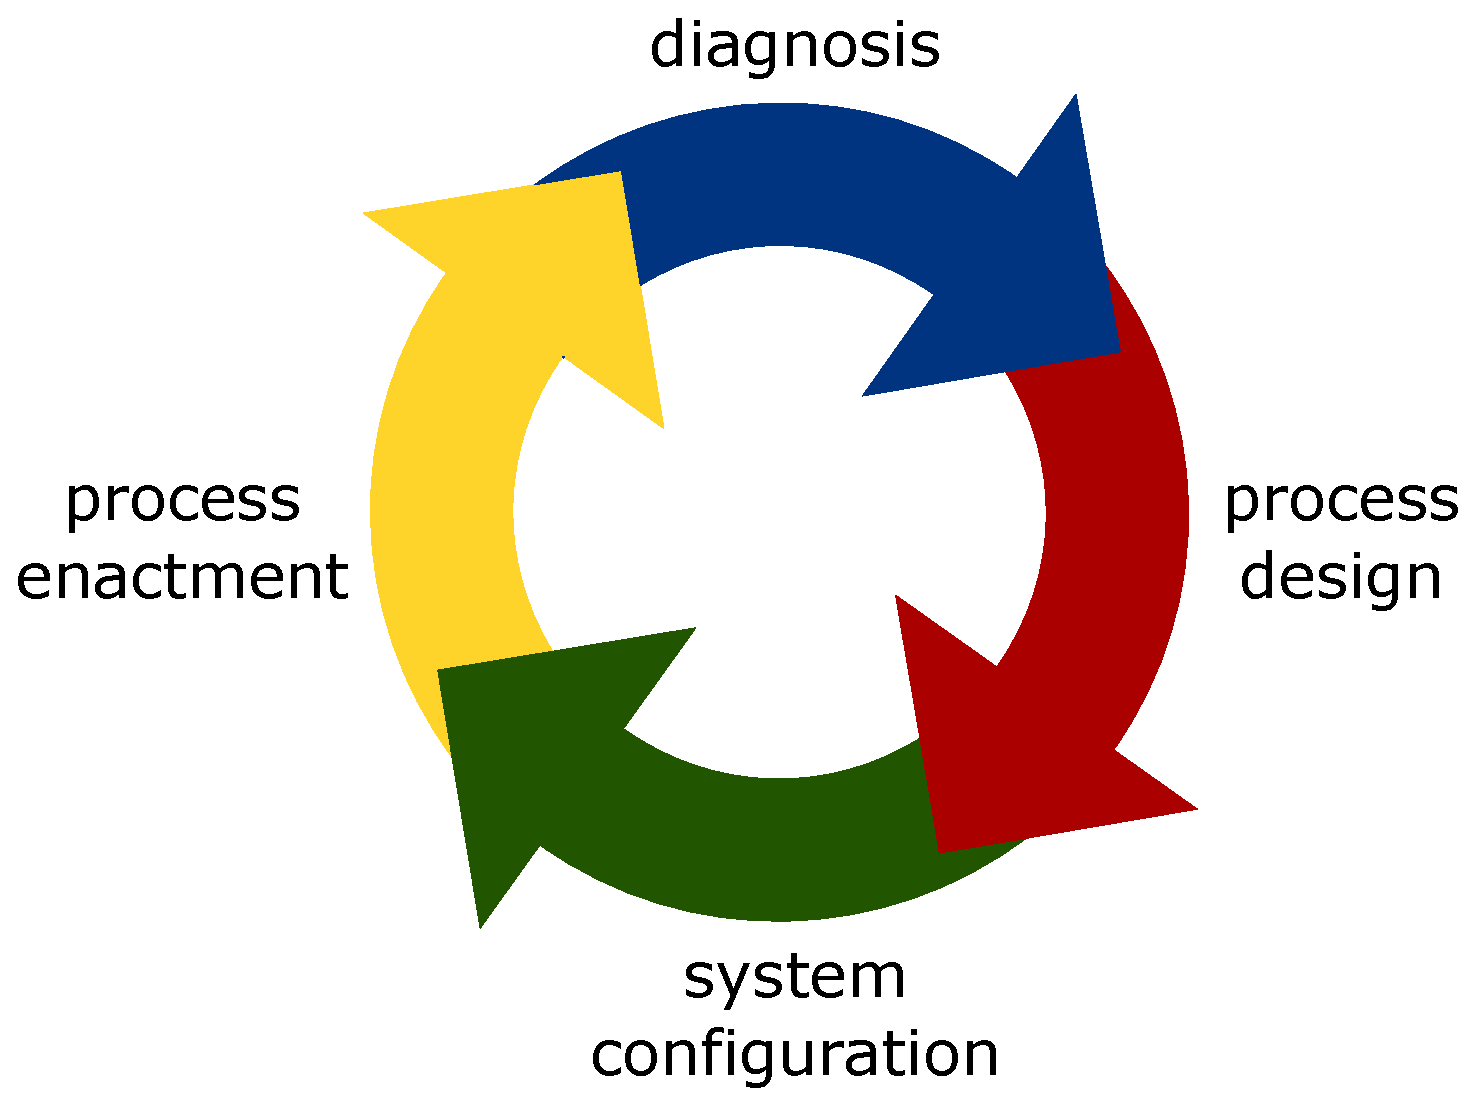
\includegraphics[width=0.5\textwidth]{Chapter1/Figs/Figure_lifecycle}
\caption[CicloVida]{Ciclo de vida del proceso de BPM Tomada de [1]}
\label{fig:CicloVida}
\end{figure}

%********************************** %Second Section  **************************************
\section{Sistemas BPM} %Section - 1.2
\label{section1.2}

Antes del surgimiento de los sistemas BPM existían los sistemas WfM, los cuales se enfocan específicamente en automatizar los procesos de negocios, dejando de lado aspectos relacionados con el control y mejoramiento de los procesos. Es por esto que los sistemas BPM tomaron relevancia, pues además de automatizar los procesos de negocios, también se enfocan en la gestión de las operaciones, la organización del trabajo, y buscan que los procesos de negocio sean más eficientes [55, 56]. Adicionalmente, tanto los sistemas BPM como los WfM, permiten obtener múltiples abstracciones de los procesos de negocio mediante la definición de flujos de trabajo o workflows \cite{VanderAalst2004}. En estos flujos de trabajo se define la secuencia de pasos a seguir en la gestión del proceso de negocio, también se definen las decisiones que se deben tomar dentro del proceso a partir de la información dada. Cada instancia de estos flujos de trabajo se denomina un ítem de trabajo o workitem, y se encarga de ejecutar la secuencia de pasos definida en la herramienta BPM teniendo en cuenta información específica. 

Es usual que para cada uno de los ítem de trabajo mencionados anteriormente se registre información relacionada con los sucesos de eventos (event logs), estos hacen referencia a eventos ocurridos dentro del proceso de ejecución de los workitems, y pueden ser almacenados de diferentes maneras, por ejemplo, en una base de datos relacional o en archivos planos. 

Dado que los procesos de negocio constantemente tienen un gran número de procesos activos, las herramientas BPM deben almacenar grandes volúmenes de información relacionada con los sucesos de eventos, al igual que deben manejar adecuadamente la concurrencia, pues es típico que en los procesos de negocio se tengan decenas de miles de elementos de trabajos activos.

Pensando en lo anterior, los sistemas WfM/BPM deben considerar ciertos aspecto importantes, no solamente los relacionados con la concurrencia, si no también los relacionados con la seguridad de la información, la seguridad del sistema, los tiempos de respuesta, la tolerancia a fallas, entre otros. De tal manera que sea posible contar con sistemas robustos y escalables, y que permitan soportar los procesos críticos de las organizaciones. Es por esto que existen algunas propuestas a nivel de arquitectura que buscan garantizar la estabilidad y robustez de las herramientas WfM/BPM [55]. 

En la actualidad existe una institución que se encarga de describir como deben funcionar los sistemas WfM/BPM, al igual de como deben ser construidos, esta entidad se llama Workflow Management Coalition (WfMC), y fue fundada en 1993 [55]. Esta institución propone un esquema de arquitectura para las herramientas BPM o WfM, de tal manera que sea posible contar con un estándar de referencia para el desarrollo y uso de estos sistemas. Algunos de los componentes más relevantes son los siguientes: 

\begin{itemize}
    \item Workflow enactment service, el cual proporciona un entorno de tiempo de ejecución que se encarga del control y la ejecución de los flujos de trabajo. Este es el componente principal de la arquitectura propuesta por el WfMC,  y puede disponer de uno o varios workflow engines, los cuales manejan partes especificas del flujo de trabajo y de los recursos del sistema [55]. 
    
    \item Process definition tools o herramientas de definición de procesos, estas herramientas permiten realizar el diseño de los procesos de negocio por medio de notación de modelado de proceso. También permiten realizar análisis y simulaciones de los procesos de negocio definidos en los flujos de trabajo [55]. 
    
    \item Workflow client applications, este componente permite a los usuarios finales comunicarse con los workflows systems, generalmente mediante el uso de los denominados in-baskets, los cuales presentan los workitems al usuario final de manera ordenada, y sobre los cuales es posible ejecutar tareas específicas.
    
    \item Administration and monitoring tools, estas herramientas de administración y monitoreo buscan controlar todo el proceso, registrando información detallada de los casos.
    
\end{itemize}

\begin{figure}[htbp!] 
\centering    
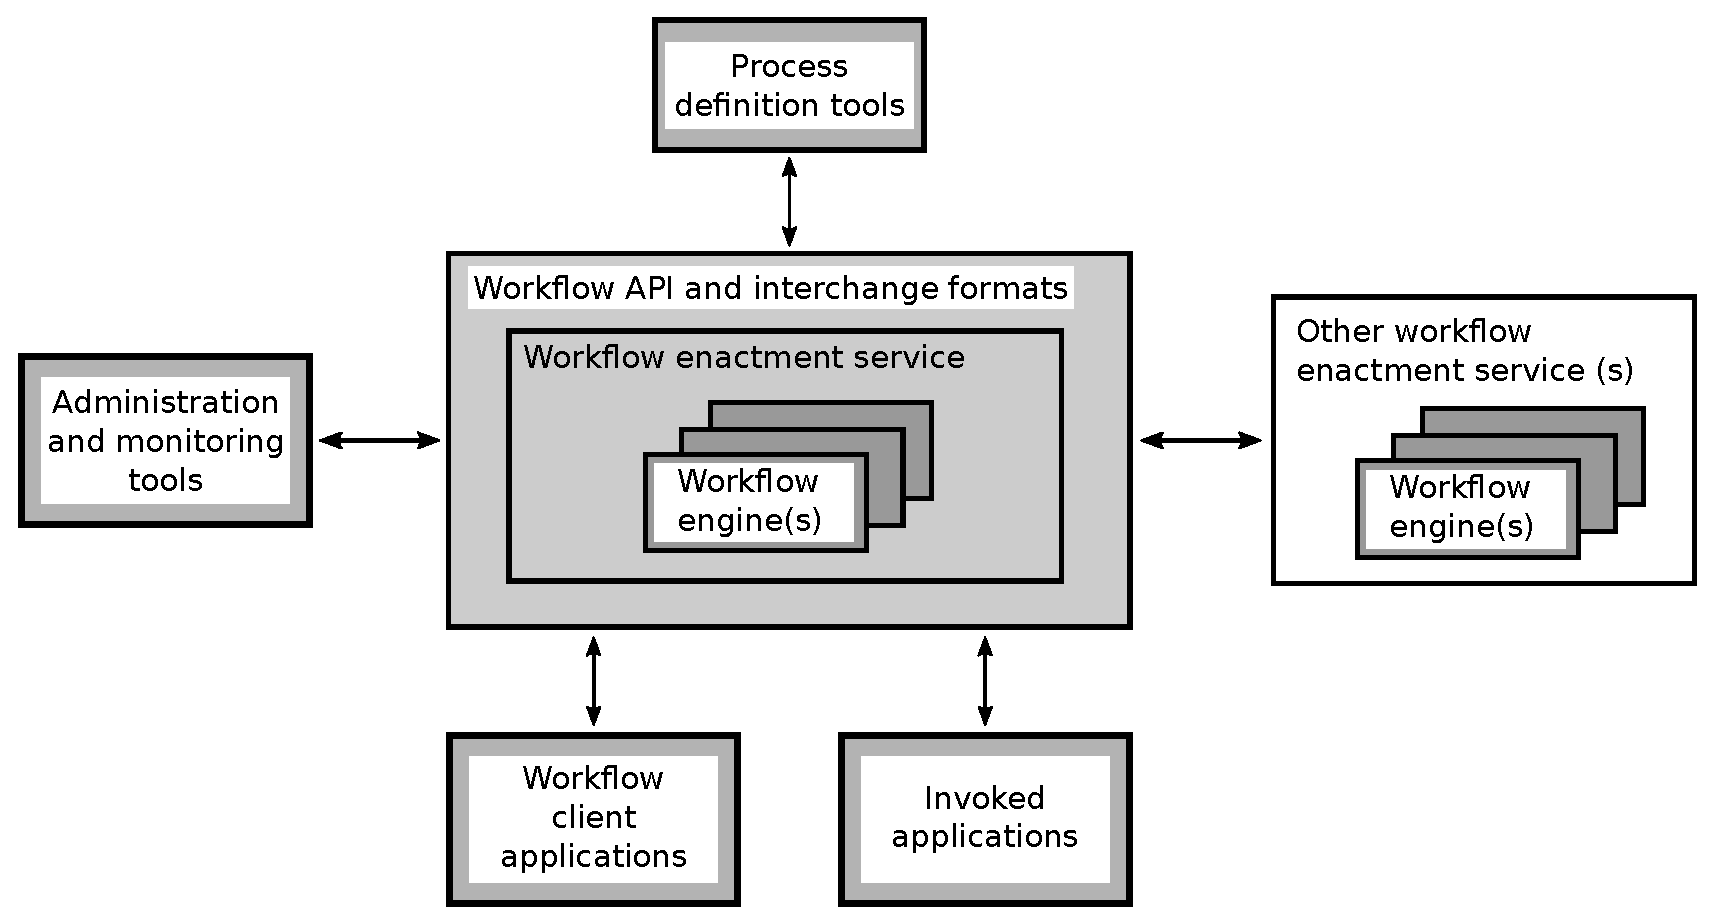
\includegraphics[width=1.0\textwidth]{Chapter1/Figs/Figure_referenceWfMC}
\caption[ReferenceWfMC]{Referencia arquitectura Tomada de [1]}
\label{fig:ReferenceWfMC}
\end{figure}

Los componentes mencionados anteriormente pueden visualizarse en las figuras [55] y (Figura 21 [55]) referencia [1], en esta última también se muestran los componentes de datos usados en los sistemas BPM, al igual que su interacción con los demás componentes.

\begin{figure}[htbp!] 
\centering    
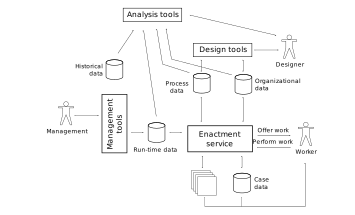
\includegraphics[width=1.0\textwidth]{Chapter1/Figs/Figure_referenceBPM}
\caption[ReferenceBPM]{Referencia arquitectura Tomada de [1]}
\label{fig:ReferenceBPM}
\end{figure}

Actualmente existen múltiples paradigmas de arquitectura, y los sistemas BPM han adoptado algunos de estos. Por ejemplo, las arquitecturas orientadas al servicio (Service Oriented Architecture SOA) han tenido un gran impacto sobre los sistemas BPM/WFM, permitiendo que los componentes sean más desacoplados y dando mas flexibilidad a las herramientas, dado que ciertos trabajos se pueden delegar o usar desde otros componentes, facilitando la integración con otros sistemas [55]. También existen arquitecturas que hacen uso de componentes cloud, las cuales pueden comprender esquemas orientados al servicio como SaaS (Sorfware as a Service), PaaS (Platform as a Services), o IaaS (Infraestructura as a Service). 

Como se puede ver, los sistemas BPM/WfM cuentan con múltiples componentes que se comunican entre sí, esta característica significa que aunque son más robustos también existen múltiples puntos de falla. Por tal razón es importante aprovechar al máximo la información generada por el sistema, y así identificar comportamiento que puedan representar una falla, esto no solo a nivel tecnológico, si no también a nivel de proceso.

\subsection{Dificultades y limitaciones en los sistemas BPM} %Section - 1.2.1
\label{section1.2.1}

Al implementar soluciones sobre la metodología BPM, surgen varias dificultades:

\begin{enumerate}
    \item El diseño de workflows puede ser un proceso complejo que consume mucho tiempo, y requiere de un conocimiento específico del proceso de negocio. Al finalizar este proceso, generalmente existen diferencias entre el workflow diseñado y el proceso real, lo que implica ajustar nuevamente la definición de los workflows [2]. Estas inconsistencias no siempre son fáciles de identificar, y frecuentemente se evidencian cuando la solución se encuentra en un ambiente productivo.
    
    \item En los sistemas BPM es usual que exista un número elevado de ítems de trabajo, como consecuencia se generan grandes volúmenes de información correspondiente al proceso de negocio y a los sucesos de eventos. Esto hace que identificar y corregir flujos que han presentado un comportamiento anómalo, ya sea a nivel de proceso de negocio o de la herramienta de software usada, sea una tarea difícil e ineficiente.
    
    \item Por otro lado, los sucesos de eventos pueden ser almacenados de una forma no estructurada o de manera incompleta, esto sumado con la gran cantidad de información generada hace que su análisis sea complejo, y no permite identificar fácilmente ciertos patrones de comportamiento que pueden ser relevantes para detectar problemas, o mejorar los procesos de negocio.
    
    \item Las herramientas de software que adoptan la metodología BPM generalmente se enfocan en analizar solamente la información de los proceso de negocio, dejando de lado la información relacionada con los sucesos de eventos presentados en los ítems de trabajo, sin embargo dicha información puede ser bastante útil. Por ejemplo, permite ajustar en una mejor medida los workflows definidos a la realidad del proceso [2]. Adicionalmente, el análisis de los sucesos de eventos podría ayudar en la caracterización y predicción de comportamientos anómalos que puedan presentarse en el proceso de negocio.
    
\end{enumerate}

En un proceso de negocio, un error o falla puede darse debido a un comportamiento anómalo en el proceso, es decir, cuando se presenta una secuencia de sucesos de eventos no esperada. Estos comportamientos pueden darse a nivel del proceso de negocio o de la plataforma, y podrían ser inferidos desde las secuencias de sucesos de eventos registradas. Comportamiento presentados en los workitems como una bifurcación no esperada dentro del proceso, la permanencia prolongada en determinado paso del proceso cuando generalmente no es así, una respuesta incorrecta o no esperada al avanzar un workitem en un paso específico, la asignación de un workitem a un usuario cuando este tipo de asignaciones no deberían ser realizadas, el inicio de un workitem por un usuario que no debería hacerlo, la finalización de un workitem padre sin que sus workitems hijos hayan finalizado, entre otros, se consideran errores o fallas del proceso de negocio. Por otro lado, errores como lentitud entre los componentes de la plataforma, respuestas de error por parte de webservices externos, fallos al ejecutar procedimientos almacenados a nivel de base de datos, errores de claves duplicadas en base de datos, privilegios insuficientes al momento de modificar un objeto dentro de la plataforma, entre otros, se consideran errores de la plataforma BPM. Estos comportamientos se dan debido a una mala gestión de los usuarios del sistema dentro del proceso, o a problemas tecnológicos.



En este contexto, la minería de procesos surge como una alternativa técnica que permite resolver las dificultades mencionadas anteriormente. Ésta se encarga de buscar modelos que permitan identificar realmente cómo trabajan las personas sobre los procesos de negocio [2], al igual que describir su comportamiento, rediseñarlos y mejorarlos continuamente [3]. Las técnicas propuestas por la minería de procesos buscan extraer información no trivial de los sucesos de eventos registrados por el sistema, y a partir de ésta, construir modelos utilizando técnicas de aprendizaje automático, lo que hace posible identificar patrones de comportamiento en los diferentes procesos de negocio [3,4]. Esta es una herramienta útil debido a que en la actualidad los procesos de negocio son cada vez más complejos y difíciles de entender, haciendo que para muchas organizaciones sea de interés realizar predicciones del comportamiento de sus procesos, particularmente los que están implementados sobre sistemas BPM o WFM (Workflow Management) [5].




%********************************** %Third Section  **************************************
\section{Minería de Procesos para la detección de fallas en sistemas BPM} %Section - 1.3
\label{section1.3}

En las organizaciones actuales, diseñar u obtener modelos de los diferentes procesos de negocio puede llegar a ser una tarea compleja, ambigua, que toma mucho tiempo y que requiere de un conocimiento profundo del negocio. La minería de procesos busca resolver estas dificultades haciendo uso de los sucesos de eventos, dado que estos contienen información detallada que permite llevar trazabilidad de cada una de las tareas ejecutadas por los procesos de negocio. Estos sucesos de eventos se registran como una secuencia de datos que generalmente contienen información del tipo de actividades u operaciones ejecutadas por cada ítem de trabajo, al igual que del tiempo de ocurrencia de estos eventos; vale la pena resaltar que estos sucesos de eventos no siempre se almacenan de una manera estructura. % Las herramientas BPM juegan un rol importante en este ámbito, pues buscan apoyar los procesos de negocio a partir de la definición de flujos de trabajo o workflows.

En este sentido, en [1] se plantea un completo manual sobre minería de procesos en el cual se analizan los diferentes patrones que pueden presentarse en los workflows, también se exponen problemas típicos de semántica que limitan el uso de la tecnología BPM o WfMS (En inglés Workflow Management Systems). En este trabajo resalta la importancia de los sistemas BPM debido a que se han convertido en una potente herramienta para la automatización de los procesos, prueba de ello es la gran cantidad de sistemas que han surgido a lo largo del tiempo.

Muchos de los trabajos realizados hasta el momento aplican técnicas de minería de procesos sobre workflows simulados, donde los datos analizados corresponden a datos de pruebas. Sin embargo en [3] por ejemplo se aplica la minería de procesos en el mundo real, donde se tiene en cuenta la información registrada por un sistema WFM, este sistema registra los sucesos de eventos necesarios para generar un modelo que permita describir el proceso; en este trabajo se puede ver que la minería de procesos no solo se aplica a sistemas de tipo WFM, sino que también se puede aplicar sobre sistemas CRM (En inglés Customer Relationship Management), ERP (En inglés Enterprise Resource Planning), entre otros, dado que estos sistemas soportan también procesos de negocio y registran sucesos de eventos.

En la actualidad existen varios trabajos en los que se abordan los retos existentes en la minería de procesos, en [22] por ejemplo se propone un algoritmo que facilita la tarea de definición de modelos de proceso a partir de sucesos de eventos; en este trabajo también se busca ampliar el uso de los sistemas que se basan en la definición de workflows, como por ejemplo los sistemas BPM. En [23] se aborda el mismo problema que en [22], pero desde el ámbito del aprendizaje automático, y haciendo uso de FWF-Net (En inglés Flexible Workflow Modeling Language), un lenguaje de modelado de workflows flexible que permite modelar y simular procesos de negocio. El algoritmo propuesto en este trabajo no solo maneja efectivamente la concurrencia en los procesos, sino que también se comporta bastante bien ante la recurrencia presentada en los mismos, este algoritmo al igual que en [22], permite transformar el resultado obtenido a una definición del workflow fácilmente. En [2] se usa la misma metodología que en [23], pero en este se propone el denominado algoritmo (alpha), el cual permite identificar nuevos modelos de proceso de negocio a partir de información de sucesos registrada por un sistema WFM, sin embargo es importante tener en cuenta que si el proceso presenta tareas ocultas, tareas duplicadas o enrutamientos complejos surgen debilidades en el algoritmo [23].

Sin embargo, a diferencia de los trabajos anteriores en los que se buscaba refinar el modelo del proceso a partir de la secuencia de eventos, en la actualidad la minería de procesos propone nuevos retos, como por ejemplo la posibilidad de predecir tiempos de completitud de las tareas o instancias de trabajo existentes [31]. En [4] se propone un método que permite predecir el futuro de una instancia de trabajo, es decir hace posible identificar el tiempo restante de ejecución de cada instancia de trabajo, o el tiempo que tomará finalizar determinada actividad. La idea básica de este trabajo es implementar un sistema de anotación de transiciones, el cual es entrenado a partir de las transacciones ejecutadas con anterioridad, con lo que es posible realizar las predicciones propuestas.

El problema de predecir la evolución de un workitem, ha llevado a la minería de procesos a usar técnicas provenientes del aprendizaje automático, específicamente técnicas que permitan modelar y clasificar secuencias de datos como las cadenas ocultas de Markov (En inglés Hidden Markov Models - HMM) [18]. Los HMM son ampliamente usados en un sinnúmero de aplicaciones de aprendizaje automático y reconocimiento de patrones, incluyendo la minería de procesos, dado que presentan buenos resultados al modelar datos secuenciales [24]. En [27] es implementado un HMM para modelar sucesos de eventos registrados por sistemas BPM o WFM. En este trabajo HMM se describe como un autómata finito donde las transiciones tienen una probabilidad asociada y los estados están asociados a un conjunto finito de salidas que cuentan con cierta probabilidad. HMM se ajusta bastante bien a los datos debido a que los procesos de negocio generalmente se pueden entender como un proceso de Markov en el cual existe una transición entre estados. En [12] se aborda el problema de la minería de procesos usando HMM como un marco de trabajo básico para un algoritmo de clasificación de secuencias, en este trabajo se evidencia un aporte significativo por parte de HMM a algoritmos de clasificación de secuencias al permitir identificar actividades paralelas, ciclos en el proceso, entre otros patrones típicos en los procesos de negocio. Teniendo en cuenta las capacidades de modelado expuestas, en [5] se aborda el mismo problema que en [4], pero haciendo uso de HMM. Se compara HMM con otros modelos estadísticos, sin embargo los autores concluyen que HMM provee mejores resultados en tareas predictivas.

Aunque los HMM han logrado buenos resultados en muchas aplicaciones, existe un problema debido a que las secuencias de datos no siempre cuentan con una distribución de tiempo constante, tal como lo supone HMM. En [28] se abarca el problema de reconocimiento de patrones sobre datos de series de tiempo en señales de onda, sin embargo debido a las debilidades presentadas por HMM al manipular datos con tiempo variable se propone una extensión de HMM, denominada HSMM (En inglés Hidden Semi-Markov Model). Este modelo elimina las distribuciones constantes o geométricas de los tiempos de duración de cada uno de los estados del proceso que generalmente son asumidas en HMM [8]. Al igual que los HMM, los HSMM han sido usados en diferentes tareas de reconocimiento de patrones [6,32], incluyendo también la minería de procesos [17]. En [17] se usa un modelo HSMM para modelar secuencias de eventos en un problema de predicción de fallas, precisamente por la capacidad de este modelo de incluir la información temporal explícita y la importancia que dicha información tiene para el problema de detección abordado. El enfoque de este trabajo es hacia la eficiencia en el procesamiento de los datos, ya que el modelo HSMM es computacionalmente mucho más costoso que el modelo HMM estándar. La solución propuesta es a nivel de hardware, permitiendo un entrenamiento mucho más rápido del modelo, pero limitando su aplicación en otros contextos ya que la solución planteada es muy específica. De manera similar, en [9] se propone el uso de HSMM para la predicción de fallas en un sistema de telecomunicaciones comercial, donde se analizan los sucesos de eventos registrados en el sistema, y se reconocen ciertos patrones de comportamiento que indican si se puede generar una falla inminente. Por otro lado, en [32] se aborda el tema de detección de intrusiones anormales en un sistema, por medio de reconocimiento de patrones usando HSMM. Para identificar dichos patrones, el modelo toma en cuenta los sucesos de eventos registrados por el sistema. Los resultados experimentales muestran que la detección de fallos depende de la longitud de la secuencia de eventos, alcanzando niveles de predicción entre el 93 y el 100 porciento, lo que permite reforzar la idea de que usar modelos HSMM en el monitoreo de sistemas en línea, puede ser un alternativa viable.

Con el objetivo de refinar y aumentar la capacidad de modelado de los HSMM, en [16] se presenta un nuevo modelo denominado NHSMM (En inglés Non-stationary Hidden Semi-Markov Model), el cual además de incorporar la información temporal de las secuencias, afina la probabilidad de transición de los estados incluyendo la dependencia del tiempo. En NHSMM se define una distribución de probabilidad de transición que permite reflejar la propiedad no estacionaria de los procesos de Markov convencionales. Al asignar una probabilidad al tiempo que dura el proceso en determinado estado, se establece que diferentes duraciones en un estado afectan la elección del nuevo estado al que se va a transitar. NHSMM no solo tiene en cuenta la duración explícita en un estado, sino que también selecciona a donde se hará la transición de acuerdo con dicha duración. Sin embargo, NHSMM no ha sido ampliamente usado, debido principalmente al costo computacional que implica su entrenamiento.

Otras técnicas de aprendizaje automático como las redes neuronales artificiales también han sido exploradas en el contexto de la minería de procesos, sin embargo estas no han alcanzado el mismo interés que los modelos antes mencionados. En [52] se hace una revisión completa de las investigaciones realizadas sobre la minería de procesos por un periodo de once años, de todos los trabajos analizados menos del dos por ciento corresponde a investigaciones que involucran las redes neuronales artificiales. En [53] se realiza un estudio exploratorio en el uso de las redes neuronales artificiales en la extracción de conocimiento a partir de procesos no estructurados, en este trabajo se evidencia que uno de los principales problemas al usar redes neuronales artificiales en la minería de procesos es la alta dimensionalidad, al igual que la pérdida semántica en la información, dado que se puede llegar a obtener un modelo que no representa el proceso analizado.

%%llevar al cpitulo de los modelos
El algoritmo de entrenamiento de los HMM, conocido como Baum-Welch (o Forward-Backward), es una implementación dinámica del algoritmo de Esperanza y Maximización (EM), el cual a su vez corresponde a una implementación del criterio de máxima verosimilitud. Generalmente EM produce buenos resultados, aunque puede sufrir de problemas de sobreajuste y puede tomar mucho tiempo en converger, particularmente para datos con una dimensionalidad alta [26]. Para un HMM estándar, con secuencias de longitud T y con N estados ocultos, la complejidad en términos de memoria del algoritmo BW crece linealmente con T y N, obteniendo una complejidad del orden O(N T ) , mientras que la complejidad respecto al tiempo crece cuadráticamente con N y linealmente con T, lo que implica una complejidad del orden de O (N 2 T ) . Estas medidas se ven fuertemente afectadas para los modelos dependientes del tiempo [9]. En una implementación sencilla de HSMM la complejidad en términos de memoria es igual a la de un HMM estándar, sin embargo la complejidad computacional durante el entrenamiento es del orden de O((N 2 + N D 2 )T ) , donde D es la máxima cantidad de tiempo que se permanece en un estado [15]. Finalmente en un NHSMM la complejidad computacional del entrenamiento es del orden de O (N 2 T D 2 ) [16].

Teniendo en cuenta la complejidad computacional de los modelos HMM y sus modificaciones, el uso de dichos modelos para resolución de problemas en el mundo real se ve limitado a la cantidad de información que es necesario procesar. Por dicha razón se han propuesto algunas alternativas que intentan reducir la complejidad computacional de los algoritmos de entrenamiento [14,31]. Otras propuestas intentan abordar dicho problema de manera paralela y/o distribuida, ya sea modificando los algoritmos de entrenamiento [47,48], o haciendo uso de herramientas especializadas en el procesamiento de información por medio de sistemas distribuidos [30]. También existen propuestas que incluyen la implementación de componentes de hardware [17,43].

Una novedosa técnica de procesamiento paralelo, y que ha tenido una gran acogida es MapReduce. Esta técnica fue desarrollada por Google, y es orientada particularmente a los problemas que involucran el procesamiento de grandes cantidades de datos [25]. Los modelos HMM pueden ser implementados bajo el paradigma de MapReduce, sinembargo es necesario ajustar los modelos a este paradigma. Por ejemplo, en [29] se muestra la aplicación de MapReduce en HSMM, donde la implementación de este modelo es realizada sobre Spark, una plataforma ampliamente usada en el contexto de Big Data.

Para el caso de los modelos NHSMM, al momento en que se realiza esta revisión, no se encuentran alternativas publicadas para la reducción de los tiempos de entrenamiento, razón por la cual aunque su capacidad de modelado es mayor que la de los modelos HMM y HSMM, como se indicó anteriormente, su uso en el contexto de la minería de procesos aún no ha sido explorado.
%%llevar al cpitulo de los modelos hasta aca

%********************************** %Fifth Section  **************************************
\section{Discusión} %Section - 1.4
\label{section1.4}

*no hay una solución para todos los casos. y lo que se pretende es evaluar que tambien se pueden realizar dechas predicciones.


%!TEX root = ../thesis.tex
%*******************************************************************************
%****************************** Second Chapter *********************************
%*******************************************************************************

\chapter{Caracterización Sucesos de Eventos}

\ifpdf
    \graphicspath{{Chapter2/Figs/Raster/}{Chapter2/Figs/PDF/}{Chapter2/Figs/}}
\else
    \graphicspath{{Chapter2/Figs/Vector/}{Chapter2/Figs/}}
\fi

Como se mencionó en el capitulo anterior, los sistemas WfM/BPM almacenan todos los sucesos de eventos generados al procesar cualquier elemento de trabajo. Estos sucesos de eventos o event logs en inglés, pueden estar relacionados por ejemplo con la creación de un nuevo elemento de trabajo, la asignación de un determinado elemento de trabajo a un usuario específico, la llegada de un elemento de trabajo a un cola específica, la invocación a un sistema externo, entre otras.

Específicamente para nuestro caso de estudio, los sucesos de eventos son almacenados en una única tabla, la cual se encuentran definida dentro de una base de datos relacional. La cantidad de registros de esta tabla crece con relación al número de elementos de trabajos procesados por el sistema, lo que quiere decir que para procesos que gestionan grandes cantidades de elementos de trabajo, se tienen grandes volúmenes de información. Esta tabla de sucesos de eventos cuenta con varios campos importantes, los cuales proveen información relevante al momento de identificar el comportamiento de los elementos de trabajo.

En vista de lo anterior, y teniendo en cuenta que, el primer paso para abordar un problema haciendo uso de la inteligencia computacional es la caracterización de la base de datos, a continuación se describirá todo el proceso llevado a cabo para realizar dicha tarea.

%********************************** %First Section  **************************************
\section{Selección de Características} %Section - 2.1 
\label{section2.1}

Al hacer uso de técnicas de machine learning o de inteligencia computacional, es usual que no sea necesario tener en cuenta todas las características de la base de datos, pues generalmente con solo algunas de estas características es posible describir adecuadamente el comportamiento de los datos. Adicional a lo anterior, tener en cuenta todas las características de la base de datos podría incrementar el costo computacional, al igual que podría hacer que los resultados obtenidos no sean los mejores. 

Para nuestro caso, se consideraron las siguientes características, las cuales fueron seleccionadas a partir del conocimiento específico de la herramienta tecnológica que las genera.


%********************************** %Second Section  **************************************
\section{One Hot Encoding} %Section - 2.2 
\label{section2.2}

Como se puede ver en la sección anterior, todas las características seleccionadas son categóricas. Lo implica que sea necesario realizar algún tipo de transformación sobre los datos, de tal manera que sea posible modelar adecuadamente los datos, al igual que aplicar las técnicas de machine leaning propuesta en este trabajo. En este orden de ideas, el mecanismo usado para realizar la categorización de los sucesos de eventos es el llamado One Hot Encoding. 

La técnica de One Hot Encoding sugiere la creación de nuevas columnas sobre la base de datos, donde cada nueva columna corresponde a una categoría de alguna de las características que componen la base de datos. Además, su valor será uno si determinado registro se encuentra asociado a dicha categoría, y en caso contrarío sería cero. La figura tal ilustra de una mejor manera lo mencionado anteriormente.  

Este proceso de One Hot Encoding da como resultado para cada registro de la base de datos un vector binario, tal como se muestra en la figura tal.

%********************************** %Third Section  **************************************
\section{Métodos de cuantización vectorial evaluados} %Section - 2.3 
\label{section2.3}

Una vez realizada la categorización de los sucesos de eventos, es necesario convertir los vectores binarios mencionados en la sección anterior a números enteros, de tal manera que sea más fácil almacenarlos y manipularlos. La figura tal muestra un ejemplo de como lucen las secuencias de sucesos de eventos después de todo el proceso realizado anteriormente. 

Sin embargo, la estructura obtenida para las secuencias de sucesos de eventos mostrada en la figura tal presentan un inconveniente, pues los valores obtenidos para cada uno de los sucesos de eventos no conforman una secuencia continua. Es por esto que debe realizarse un proceso denominado cuantización vectorial sobre los nuevos datos obtenidos. Este proceso busca que los nuevos datos sean almacenados de la forma más compacta posible, y también que sean representados con suficiente precisión, de tal manera que sea posible generar una secuencia continua con dichas observaciones [51]. Agregar figura. 

Generalmente, este proceso de cuantización vectorial se lleva a cabo haciendo uso de técnicas o métodos de clasificación. En la literatura se ha encontrado que el método más usado es el K-means. Sin embargo, la condición de los datos que se están modelando en este trabajo suponen una dificultad, pues las observaciones obtenidas corresponden a vectores binarios, sobre los cuales no se puede aplicar una medida de distancia como la euclidiana, y por el contrario es necesario usar la distancia hamming. 

Debido a que tal vez los resultados obtenidos con la técnica de K-means y la distancia hamming no sean los mejores, se hace uso también de la técnica de K-mode, la cual toma en cuenta la moda de las distancias de los diferentes puntos. Esta técnica es comúnmente usada para clasificar secuencias genéticas.   

En conclusión, dentro del proceso de cuantización de los datos se tuvieron en cuenta tres métodos. El método de K-means, el método de K-moda, y por último, un método que no hace uso de técnicas de clasificación, pero que le asigna un único identificador a cada observación.


%llever a la seccion de entrenamiento e implementación
es necesario generar las secuencias de sucesos de eventos, con estas secuencias se podrán identificar patrones en el comportamiento de los work items. Esto es importante debido que se esta abordando un problema relacionado con aprendizaje estructura, es decir que existen una dependencia entre cada nuevo suceso de evento con el anterior. Adicional, esta sería la estructura que soportan los modelos que son implementados para este trabajo.

Varias tareas se deben tener en cuenta para generar dichas secuencias de sucesos, primero se deben separar las secuencias que están asociadas a un error con las secuencias que no lo están, luego a partir de la característica de tiempo se ordenan los registros y se genera la secuencias con orden temporal. Para nuestro caso se estudio, la longitud de las secuencias pueden variar bastante, puedes existir secuencias muy pequeñas, pero también secuencias muy extensas, el maximo de observaciones es hasta de seis mil.
La sigueinte figura ilustra el proceso de generación de las secuencias de sucesos. Figura
%hasta acá



%********************************** %Quarter Section  **************************************
\section{Métodos de cuantización vectorial evaluados} %Section - 2.4 
\label{section2.4}



%!TEX root = ../thesis.tex
%*******************************************************************************
%****************************** Third Chapter **********************************
%*******************************************************************************
\chapter{Costo computacional e Implementación del sistema de detección de fallas}

% **************************** Define Graphics Path **************************
\ifpdf
    \graphicspath{{Chapter3/Figs/Raster/}{Chapter3/Figs/PDF/}{Chapter3/Figs/}}
\else
    \graphicspath{{Chapter3/Figs/Vector/}{Chapter3/Figs/}}
\fi

%********************************** %First Section  **************************************
\section{Costo computacional de los modelos} %Section - 3.1 
\label{section3.1}


La principal dificultad que se tienen al trabajar modelos de estados ocultos de markov es el alto costo computacional, y que este crece exponencialmente al aumentar el numero de secuencias a analizar, al igual que al aumentar los parametros del modelo. A continuación se describirá el costo computacional teorico para cada modelo. 




Lo anterior hace evidente que sea necesario plantear un mecanismo que permita entrenar los modelos de manera eficiente, por tal rezon se ha propuesto usar spark para dicha tarea, con spark es posible distribuir la carga de trabajo en disferentes nodos del cluster, de tal manera que se puedan obtner resultados en un menor tiempo. 

%********************************** %Second Section  **************************************
\section{Estrategia de paralelización para los modelos HMM; HSMM, NHSMM } %Section - 3.2 
\label{section3.2}

En spark la estrcutura usada para manipular los datos es la estructura de dataframe, la blablabla

LA idea de usar sparl es poder distribuir el trabajo en diferentes nodos del cluster, por tal razon se hizo uso de algunas estrategias de paralelización, 
primero se uso la función de repartition, esta función permite bla bla bla, imagen

también se usaron funciones UDF, imagen

Y finalmente se usaron las funciones de reduce, imagen


Especificar un poco sin agregar codigo



%********************************** %Third Section  **************************************
\section{Estrategia de paralelización para los modelos LJTM} %Section - 3.3 
\label{section3.3}




\subsection{Second subsection in the first section}
\dots and some more \dots

\subsubsection{First subsub section in the second subsection}
\dots and some more in the first subsub section otherwise it all looks the same
doesn't it? well we can add some text to it \dots

\subsection{Third subsection in the first section}
\dots and some more \dots

\subsubsection{First subsub section in the third subsection}
\dots and some more in the first subsub section otherwise it all looks the same
doesn't it? well we can add some text to it and some more and some more and
some more and some more and some more and some more and some more \dots

\subsubsection{Second subsub section in the third subsection}
\dots and some more in the first subsub section otherwise it all looks the same
doesn't it? well we can add some text to it \dots

\section{Second section of the third chapter}
and here I write more \dots

\section{The layout of formal tables}
This section has been modified from ``Publication quality tables in \LaTeX*''
 by Simon Fear.

The layout of a table has been established over centuries of experience and 
should only be altered in extraordinary circumstances. 

When formatting a table, remember two simple guidelines at all times:

\begin{enumerate}
  \item Never, ever use vertical rules (lines).
  \item Never use double rules.
\end{enumerate}

These guidelines may seem extreme but I have
never found a good argument in favour of breaking them. For
example, if you feel that the information in the left half of
a table is so different from that on the right that it needs
to be separated by a vertical line, then you should use two
tables instead. Not everyone follows the second guideline:

There are three further guidelines worth mentioning here as they
are generally not known outside the circle of professional
typesetters and subeditors:

\begin{enumerate}\setcounter{enumi}{2}
  \item Put the units in the column heading (not in the body of
          the table).
  \item Always precede a decimal point by a digit; thus 0.1
      {\em not} just .1.
  \item Do not use `ditto' signs or any other such convention to
      repeat a previous value. In many circumstances a blank
      will serve just as well. If it won't, then repeat the value.
\end{enumerate}

A frequently seen mistake is to use `\textbackslash begin\{center\}' \dots `\textbackslash end\{center\}' inside a figure or table environment. This center environment can cause additional vertical space. If you want to avoid that just use `\textbackslash centering'


\begin{table}
\caption{A badly formatted table}
\centering
\label{table:bad_table}
\begin{tabular}{|l|c|c|c|c|}
\hline 
& \multicolumn{2}{c}{Species I} & \multicolumn{2}{c|}{Species II} \\ 
\hline
Dental measurement  & mean & SD  & mean & SD  \\ \hline 
\hline
I1MD & 6.23 & 0.91 & 5.2  & 0.7  \\
\hline 
I1LL & 7.48 & 0.56 & 8.7  & 0.71 \\
\hline 
I2MD & 3.99 & 0.63 & 4.22 & 0.54 \\
\hline 
I2LL & 6.81 & 0.02 & 6.66 & 0.01 \\
\hline 
CMD & 13.47 & 0.09 & 10.55 & 0.05 \\
\hline 
CBL & 11.88 & 0.05 & 13.11 & 0.04\\ 
\hline 
\end{tabular}
\end{table}

\begin{table}
\caption{A nice looking table}
\centering
\label{table:nice_table}
\begin{tabular}{l c c c c}
\hline 
\multirow{2}{*}{Dental measurement} & \multicolumn{2}{c}{Species I} & \multicolumn{2}{c}{Species II} \\ 
\cline{2-5}
  & mean & SD  & mean & SD  \\ 
\hline
I1MD & 6.23 & 0.91 & 5.2  & 0.7  \\

I1LL & 7.48 & 0.56 & 8.7  & 0.71 \\

I2MD & 3.99 & 0.63 & 4.22 & 0.54 \\

I2LL & 6.81 & 0.02 & 6.66 & 0.01 \\

CMD & 13.47 & 0.09 & 10.55 & 0.05 \\

CBL & 11.88 & 0.05 & 13.11 & 0.04\\ 
\hline 
\end{tabular}
\end{table}


\begin{table}
\caption{Even better looking table using booktabs}
\centering
\label{table:good_table}
\begin{tabular}{l c c c c}
\toprule
\multirow{2}{*}{Dental measurement} & \multicolumn{2}{c}{Species I} & \multicolumn{2}{c}{Species II} \\ 
\cmidrule{2-5}
  & mean & SD  & mean & SD  \\ 
\midrule
I1MD & 6.23 & 0.91 & 5.2  & 0.7  \\

I1LL & 7.48 & 0.56 & 8.7  & 0.71 \\

I2MD & 3.99 & 0.63 & 4.22 & 0.54 \\

I2LL & 6.81 & 0.02 & 6.66 & 0.01 \\

CMD & 13.47 & 0.09 & 10.55 & 0.05 \\

CBL & 11.88 & 0.05 & 13.11 & 0.04\\ 
\bottomrule
\end{tabular}
\end{table}

%!TEX root = ../thesis.tex
%*******************************************************************************
%****************************** Quarter Chapter *********************************
%*******************************************************************************

\chapter{Implementación y programación distribuida}

\ifpdf
    \graphicspath{{Chapter4/Figs/Raster/}{Chapter4/Figs/PDF/}{Chapter4/Figs/}}
\else
    \graphicspath{{Chapter4/Figs/Vector/}{Chapter4/Figs/}}
\fi


%********************************** %First Section  **************************************
\section{Entrenamiento, validación y predicción de los modelos} %Section - 4.1 
\label{section4.1}

Como se mencionó en el capitulo dos, por cada elemento de trabajo se tiene una secuencia de suscesos, estas secuencias de sucesos tienen una longitud variable, y son almacenados en un dataframe con dos columnas, la primera indica el id del elemento de trabajo, y la segunda corresonde a la secuencias de proceso. A dicional a esta estructura se debe tener encuenta que las secuencias de suscesos estas clasificadas, es decir se tiene un conjunto de secuencias correspondientes a los elementos de trabajo que fallaron en la herramienta WfM, y se tiene otro conjunto de secuencias que no fallaron. Teniendo esta distinción se puede iniciar con el proceso de entrenamiento. Es importance mencionar que estos satoso involucran un problema estructural, esto debido a que existe una dependencia entre observaciones, siempre la siguiente depende de la anterior.

Para cada modelo que se valido, se realizó el entrenamiento de cada conjunto de datos, haciendo uso de las crosvalidation con 5 folds, a partir de esto se realizó el calculo de los indicadores que permiten determinar cuales son los mejores parametros para el modelo.

Luego de esto, es posible realizar la evalución de la capacidad de predicción de los modelos, dado que los modelos han sido almacenados previamente, ahora con esto es posible calcular a partir de la longitud de las secuencias el poder de predicción de los modelos, ....

Agregar figura flujo del proceso.



%********************************** %Second Section  **************************************
\section{Implementación de los algoritmos } %Section - 4.2 
\label{section4.2}

LA implementación de los modelos HMM y demas consiste basicamente en definir aleatoriamente los parametros del modelo, que son las matrices A, B, pi, una vez se tienen esotos valores se empieza con el procesamiento, es decir el forwar y el back, este procesos, 

codigo relevante para la implementación y librerías relevantes, blablabla



%********************************** %Third Section  **************************************
\section{Programación distribuida} %Section - 4.3 
\label{section4.3}

Dado que el proceso secuencial es tan deficiente, se procede con el uso de tecnicas de programación distribuidas, como sparl, blblblb donde se usa el repartitions, y el reduce, los cuales eficiente menet reducen considerablemente el rpceoso, tamién se almacenas la info para poder ejecutar procesos de recovery, bablalblb

%!TEX root = ../thesis.tex
%*******************************************************************************
%****************************** Fifth Chapter *********************************
%*******************************************************************************

\chapter{Experimentos y Resultados}

\ifpdf
    \graphicspath{{Chapter5/Figs/Raster/}{Chapter5/Figs/PDF/}{Chapter5/Figs/}}
\else
    \graphicspath{{Chapter5/Figs/Vector/}{Chapter5/Figs/}}
\fi

%********************************** %First Section  **************************************
\section{Resultados para HMM} %Section - 5.1 
\label{section5.1}

%********************************** %Second Section  **************************************
\section{Resultados para HSMM} %Section - 5.2 
\label{section5.2}

%********************************** %Third Section  **************************************
\section{Resultados para NHSMM} %Section - 5.3 
\label{section5.3}

%********************************** %Third Section  **************************************
\section{Resultados para LSTM} %Section - 5.4 
\label{section5.4}

%!TEX root = ../thesis.tex
%*******************************************************************************
%*********************************** Conclusions ******************************
%*******************************************************************************

\chapter*{Conclusiones} 
\addcontentsline{toc}{chapter}{Conclusiones}
%\include{Chapter6/chapter6}
%\include{Chapter7/chapter7}



% ********************************** Back Matter *******************************
% Backmatter should be commented out, if you are using appendices after References
%\backmatter

% ********************************** Bibliography ******************************
\begin{spacing}{0.9}

% To use the conventional natbib style referencing
% Bibliography style previews: http://nodonn.tipido.net/bibstyle.php
% Reference styles: http://sites.stat.psu.edu/~surajit/present/bib.htm

\bibliographystyle{apalike}
%\bibliographystyle{unsrt} % Use for unsorted references  
%\bibliographystyle{plainnat} % use this to have URLs listed in References
\cleardoublepage
\bibliography{References/references} % Path to your References.bib file


% If you would like to use BibLaTeX for your references, pass `custombib' as
% an option in the document class. The location of 'reference.bib' should be
% specified in the preamble.tex file in the custombib section.
% Comment out the lines related to natbib above and uncomment the following line.

%\printbibliography[heading=bibintoc, title={References}]


\end{spacing}

% ********************************** Appendices ********************************

\begin{appendices} % Using appendices environment for more functunality

% %!TEX root = ../thesis.tex
% ******************************* Thesis Appendix A ****************************
\chapter{How to install \LaTeX} 

\section*{Windows OS}

\subsection*{TeXLive package - full version}
\begin{enumerate}
\item	Download the TeXLive ISO (2.2GB) from\\
\href{https://www.tug.org/texlive/}{https://www.tug.org/texlive/}
\item	Download WinCDEmu (if you don't have a virtual drive) from \\
\href{http://wincdemu.sysprogs.org/download/}
{http://wincdemu.sysprogs.org/download/}
\item	To install Windows CD Emulator follow the instructions at\\
\href{http://wincdemu.sysprogs.org/tutorials/install/}
{http://wincdemu.sysprogs.org/tutorials/install/}
\item	Right click the iso and mount it using the WinCDEmu as shown in \\
\href{http://wincdemu.sysprogs.org/tutorials/mount/}{
http://wincdemu.sysprogs.org/tutorials/mount/}
\item	Open your virtual drive and run setup.pl
\end{enumerate}

or

\subsection*{Basic MikTeX - \TeX~ distribution}
\begin{enumerate}
\item	Download Basic-MiK\TeX (32bit or 64bit) from\\
\href{http://miktex.org/download}{http://miktex.org/download}
\item	Run the installer 
\item	To add a new package go to Start >> All Programs >> MikTex >> Maintenance (Admin) and choose Package Manager
\item	Select or search for packages to install
\end{enumerate}

\subsection*{TexStudio - \TeX~ editor}
\begin{enumerate}
\item	Download TexStudio from\\
\href{http://texstudio.sourceforge.net/\#downloads}
{http://texstudio.sourceforge.net/\#downloads} 
\item	Run the installer
\end{enumerate}

\section*{Mac OS X}
\subsection*{MacTeX - \TeX~ distribution}
\begin{enumerate}
\item	Download the file from\\
\href{https://www.tug.org/mactex/}{https://www.tug.org/mactex/}
\item	Extract and double click to run the installer. It does the entire configuration, sit back and relax.
\end{enumerate}

\subsection*{TexStudio - \TeX~ editor}
\begin{enumerate}
\item	Download TexStudio from\\
\href{http://texstudio.sourceforge.net/\#downloads}
{http://texstudio.sourceforge.net/\#downloads} 
\item	Extract and Start
\end{enumerate}


\section*{Unix/Linux}
\subsection*{TeXLive - \TeX~ distribution}
\subsubsection*{Getting the distribution:}
\begin{enumerate}
\item	TexLive can be downloaded from\\
\href{http://www.tug.org/texlive/acquire-netinstall.html}
{http://www.tug.org/texlive/acquire-netinstall.html}.
\item	TexLive is provided by most operating system you can use (rpm,apt-get or yum) to get TexLive distributions
\end{enumerate}

\subsubsection*{Installation}
\begin{enumerate}
\item	Mount the ISO file in the mnt directory
\begin{verbatim}
mount -t iso9660 -o ro,loop,noauto /your/texlive####.iso /mnt
\end{verbatim}

\item	Install wget on your OS (use rpm, apt-get or yum install)
\item	Run the installer script install-tl.
\begin{verbatim}
	cd /your/download/directory
	./install-tl
\end{verbatim}
\item	Enter command `i' for installation

\item	Post-Installation configuration:\\
\href{http://www.tug.org/texlive/doc/texlive-en/texlive-en.html\#x1-320003.4.1}
{http://www.tug.org/texlive/doc/texlive-en/texlive-en.html\#x1-320003.4.1} 
\item	Set the path for the directory of TexLive binaries in your .bashrc file
\end{enumerate}

\subsubsection*{For 32bit OS}
For Bourne-compatible shells such as bash, and using Intel x86 GNU/Linux and a default directory setup as an example, the file to edit might be \begin{verbatim}
edit $~/.bashrc file and add following lines
PATH=/usr/local/texlive/2011/bin/i386-linux:$PATH; 
export PATH 
MANPATH=/usr/local/texlive/2011/texmf/doc/man:$MANPATH;
export MANPATH 
INFOPATH=/usr/local/texlive/2011/texmf/doc/info:$INFOPATH;
export INFOPATH
\end{verbatim}
\subsubsection*{For 64bit OS}
\begin{verbatim}
edit $~/.bashrc file and add following lines
PATH=/usr/local/texlive/2011/bin/x86_64-linux:$PATH;
export PATH 
MANPATH=/usr/local/texlive/2011/texmf/doc/man:$MANPATH;
export MANPATH 
INFOPATH=/usr/local/texlive/2011/texmf/doc/info:$INFOPATH;
export INFOPATH

\end{verbatim}



%\subsection{Installing directly using Linux packages} 
\subsubsection*{Fedora/RedHat/CentOS:}
\begin{verbatim} 
sudo yum install texlive 
sudo yum install psutils 
\end{verbatim}


\subsubsection*{SUSE:}
\begin{verbatim}
sudo zypper install texlive
\end{verbatim}


\subsubsection*{Debian/Ubuntu:}
\begin{verbatim} 
sudo apt-get install texlive texlive-latex-extra 
sudo apt-get install psutils
\end{verbatim}

% %!TEX root = ../thesis.tex
% ******************************* Thesis Appendix B ********************************

\chapter{Installing the CUED class file}

\LaTeX.cls files can be accessed system-wide when they are placed in the
<texmf>/tex/latex directory, where <texmf> is the root directory of the user’s \TeX installation. On systems that have a local texmf tree (<texmflocal>), which
may be named ``texmf-local'' or ``localtexmf'', it may be advisable to install packages in <texmflocal>, rather than <texmf> as the contents of the former, unlike that of the latter, are preserved after the \LaTeX system is reinstalled and/or upgraded.

It is recommended that the user create a subdirectory <texmf>/tex/latex/CUED for all CUED related \LaTeX class and package files. On some \LaTeX systems, the directory look-up tables will need to be refreshed after making additions or deletions to the system files. For \TeX Live systems this is accomplished via executing ``texhash'' as root. MIK\TeX users can run ``initexmf -u'' to accomplish the same thing.

Users not willing or able to install the files system-wide can install them in their personal directories, but will then have to provide the path (full or relative) in addition to the filename when referring to them in \LaTeX.

\end{appendices}

% *************************************** Index ********************************
\printthesisindex % If index is present

\end{document}
